% Copyright 2004 by Till Tantau <tantau@users.sourceforge.net>.
%
% In principle, this file can be redistributed and/or modified under
% the terms of the GNU Public License, version 2.
%
% However, this file is supposed to be a template to be modified
% for your own needs. For this reason, if you use this file as a
% template and not specifically distribute it as part of a another
% package/program, I grant the extra permission to freely copy and
% modify this file as you see fit and even to delete this copyright
% notice. 

\documentclass{beamer}
% Replace the \documentclass declaration above
% with the following two lines to typeset your 
% lecture notes as a handout:
%\documentclass{article}
%\usepackage{beamerarticle}

\usepackage{graphicx}
\usepackage[utf8]{inputenc}
\usepackage{tabto}
 
\graphicspath{ {img/} }


% There are many different themes available for Beamer. A comprehensive
% list with examples is given here:
% http://deic.uab.es/~iblanes/beamer_gallery/index_by_theme.html
% You can uncomment the themes below if you would like to use a different
% one:
%\usetheme{AnnArbor}
%\usetheme{Antibes}
%\usetheme{Bergen}
%\usetheme{Berkeley}
%\usetheme{Berlin}
%\usetheme{Boadilla}
%\usetheme{boxes}
%\usetheme{CambridgeUS}
%\usetheme{Copenhagen}
%\usetheme{Darmstadt}
%\usetheme{default}
%\usetheme{Frankfurt}
%\usetheme{Goettingen}
%\usetheme{Hannover}
%\usetheme{Ilmenau}
%\usetheme{JuanLesPins}
%\usetheme{Luebeck}
%\usetheme{Madrid}
%\usetheme{Malmoe}
%\usetheme{Marburg}
%\usetheme{Montpellier}
%\usetheme{PaloAlto}
%\usetheme{Pittsburgh}
%\usetheme{Rochester}
%\usetheme{Singapore}
%\usetheme{Szeged}
\usetheme{Warsaw}

\title{Programming with Python}

% A subtitle is optional and this may be deleted
\subtitle{Lesson 2: Conditionals and Loops}

%\author{F.~Author\inst{1} \and S.~Another\inst{2}}
% - Give the names in the same order as the appear in the paper.
% - Use the \inst{?} command only if the authors have different
%   affiliation.

%\institute[Universities of Somewhere and Elsewhere] % (optional, but mostly needed)
%{
%  \inst{1}%
%  Department of Computer Science\\
%  University of Somewhere
%  \and
%  \inst{2}%
%  Department of Theoretical Philosophy\\
%  University of Elsewhere}
% - Use the \inst command only if there are several affiliations.
% - Keep it simple, no one is interested in your street address.

\date{November 8th, 2016}
% - Either use conference name or its abbreviation.
% - Not really informative to the audience, more for people (including
%   yourself) who are reading the slides online

\subject{Python Lessons}
% This is only inserted into the PDF information catalog. Can be left
% out. 

% If you have a file called "university-logo-filename.xxx", where xxx
% is a graphic format that can be processed by latex or pdflatex,
% resp., then you can add a logo as follows:

% \pgfdeclareimage[height=0.5cm]{university-logo}{university-logo-filename}
% \logo{\pgfuseimage{university-logo}}

% Delete this, if you do not want the table of contents to pop up at
% the beginning of each subsection:
%\AtBeginSubsection[]
%{
%  \begin{frame}<beamer>{Outline}
%    \tableofcontents[currentsection,currentsubsection]
%  \end{frame}
%}

% Let's get started
\begin{document}

\begin{frame}
  \titlepage
\end{frame}

%\begin{frame}{Outline}
%  \tableofcontents
%  % You might wish to add the option [pausesections]
%\end{frame}

% Section and subsections will appear in the presentation overview
% and table of contents.
\section{Introduction \& Recap}

\begin{frame}{Last week's goals}
\pause
\begin{itemize}
  \item We installed Python and PyCharm
  \pause
  \item We learnt about variables and variable types
  \pause
  \item We learnt about printing and asking for input from the user
  \pause
  \item And we made a simple adding calculator
  \end{itemize}

\pause

\begin{figure}[h]
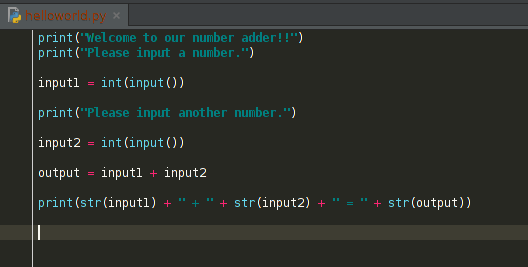
\includegraphics[width=0.5\textwidth]{calc}
\end{figure}

\end{frame}

\begin{frame}{Problems with our calculator}
What is wrong with our calculator right now?

\pause

\begin{itemize}
  \item It can only add
  \pause
  \item It breaks when you don't give it a number
  \pause
  \item It adds two numbers then finishes
\end{itemize}

\pause

We are going to soup up our calculator to fix all these bugs!

\end{frame}

\section{Conditionals}

\begin{frame}{What's a conditional? What's a boolean?}

\pause

\begin{figure}[h]

\includegraphics[width=0.5\textwidth]{yes}
\caption{image curtosy of ArtsyBee from http://pixabay.com}
\end{figure}


\end{frame}

\begin{frame}{Boolean type \& operators}

Boolean can be one of two values in Python:
\pause
\begin{itemize}
  \item True
  \item False
\end{itemize}

\pause

There are also a bunch of operators to compare booleans
\pause
\begin{itemize}
  \item[] \textgreater  : Greater than
  \pause
  \item[] \textgreater =  : Greater than or equal to
  \pause
  \item[] \textless  : Less than
  \pause
  \item[] \textless =  : Less than or equal to
  \pause
  \item[] == : Equal to
  \pause
  \item[] != : Not equal to
\end{itemize}


\end{frame}

\begin{frame}{Some examples}
\pause
\begin{itemize}
  \item[] 4 == 3? \pause \tab False
  \pause
  \item[] 4 \textgreater = 3? \pause \tab True
  \pause
  \item[] 4 == "Hello World!"? \pause \tab False
  \pause
  \item[] True != True? \pause \tab False
  \pause
  \item[] 4 == (4 == 4)? \pause \tab False... why?
\end{itemize}

\end{frame}

\begin{frame}{MORE boolean operators}
\pause
\begin{itemize}
  \item[] and : And
  \pause
  \item[] or : Or
  \pause
  \item[] ! : Negate
\end{itemize}
\end{frame}

\begin{frame}{More examples}
\pause
\begin{itemize}
  \item[] (4 == 3) or (4 == 4)? \pause \tab True
  \pause
  \item[] ("Casper" != "Is Cool") and ("Jonathan" != "Is Cool") \pause \tab True
  \pause
  \item[] 3 == 3 and (not ("testing" == "testing" or "Python" == "Fun")) \pause \tab False
\end{itemize}

\end{frame}

\begin{frame}{The 'if' statement}

Three basic formats in python:
\pause
\begin{enumerate}

  \item if(BOOLEAN):\\
            \qquad thing\\
  \pause
  \item if(BOOLEAN):\\
            \qquad thing\\
        else:\\
            \qquad other thing
  \pause
  \item if(BOOLEAN):\\
            \qquad thing\\
        elif(BOOLEAN):\\
            \qquad other thing\\
        else:\\
            \qquad Yet another other thing
  

\end{enumerate}

\end{frame}


\begin{frame}{For example...}

\begin{figure}[h]
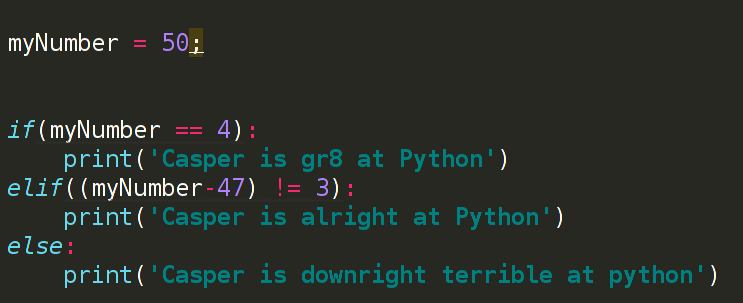
\includegraphics[width=0.9\textwidth]{exampleif}
\end{figure}

\pause

Can anyone guess what it says?

\end{frame}



\begin{frame}{Back to the calculator}

How can we extend our calculator to add, subtract, divide and multiply?
\pause
Time for some live coding!

\end{frame}

\section{Handling Errors}

\begin{frame}
Our calculator is beginning to take shape!
\pause
However, what can go wrong with our calculator?
\pause
How can we deal with our errors?

\end{frame}

\begin{frame}{Handling our errors}

More live coding!

\end{frame}

\section{Looping}

\begin{frame}{Our calculator just gets better and better}

What now?\\
\pause
Lets make sure the user enters the correct operation, without having to restart the program!

\end{frame}

\begin{frame}{Looping}

What are loops?
\pause
What different kind of loops are there?

\end{frame}

\begin{frame}{The while loop}
while(BOOLEAN):\\
            \qquad something\\
            \qquad something else\\
\end{frame}

\begin{frame}{An example}
\begin{figure}[h]
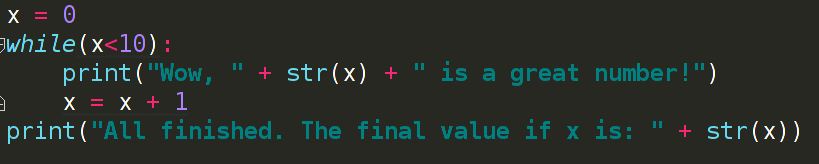
\includegraphics[width=0.9\textwidth]{examplewhile}
\end{figure}
\end{frame}

\begin{frame}{An example}
\begin{figure}[h]
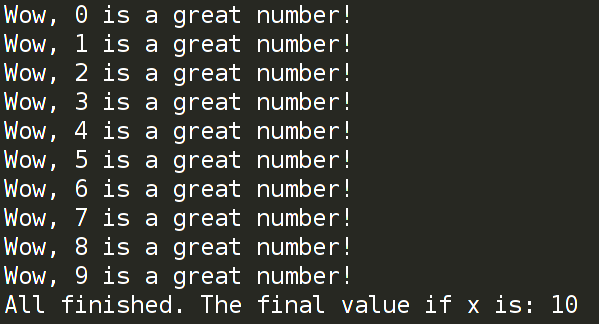
\includegraphics[width=0.8\textwidth]{whileoutput}
\end{figure}

\pause
What would happen without the x = x + 1 line?\\

\pause
What would happen if the x = x + 1 line was before the print?

\end{frame}

\begin{frame}
Yet more live coding!
\end{frame}

\begin{frame}

Our calculator is looking pretty sweet now.\\
\pause
However, we still have to re-run the program every time we want to do another calculation.\\ \pause What can we do about this?
\end{frame}

\begin{frame}
A final little bit more of live coding!
\end{frame}


\begin{frame}{That's all for tonight}
  To summarise:
  \begin{itemize}
  \item We have learnt about conditionals
  \item We have used conditionals to make our calculator be able to add, subtract, divide or multiply
  \item We have used conditionals to handle errors
  \item We have learnt about loops and used them to make our program much more usable
  \end{itemize}
\end{frame}

\begin{frame}{For next week}
Source code plus lecture slides will be available online soon after the lesson.\\
If you are new to HackSocNotts, please join us on \textit{http://hacksocnotts.slack.com}.\\
If you have any questions, feel free to ask now or over slack.\\
\end{frame}

\end{document}


